\section{Sicherungsschicht}

\paragraph{Terminologie}
\begin{items}
  \item \textbf{Knoten}: Endsysteme + Router
  \item \textbf{Links}: Übertragungsabschnitt zwischen benachbarten Knoten
  \item \textbf{Rahmen}: Pakete auf Schicht 2 (IP-Datagramme eingekapselt)
  \item \textbf{Aufgabe}: Übertragung von Datagrammen zwischen benachbarten Knoten über Link
\end{items}

\paragraph{Aufgaben}
\begin{items}
  \item \textbf{Strukturierung} des Datenstroms (\emph{framing}) \\*
    \( \leadsto \) Datagramm in Rahmen einkapseln hinzufügen
  \item \textbf{Medienzugangskontrolle} bei geteilten Medien
  \item \textbf{Adressierung} mittels MAC-Adressen
  \item Je nach angebotenem Dienst \emph{Fehlererkennung/-behebung} bzw. \emph{Flusskontrolle}
	\medskip
  \item \textbf{(Semi-) Broadcast}: Alle Stationen sehen alle Rahmen (zB WLAN = semi-broadcast)
  \item \textbf{Punkt-zu-Punkt-Link}: Zwei Stationen sind über dedizierten Link verbunden \\*
  	 (zB switch-basiertes Ethernet)\\*
	  - \emph{Simplex}: Übertragung in eine Richtung\\*
  	  - \emph{Halbduplex}: Übertragung in beide Richtungen, nicht zeitgleich\\*
      - \emph{(Voll-) Duplex}: Übertragung in beide Richtungen, zeitgleich
\end{items}

\paragraph{Sicherungsschicht --- Implementierung}
\begin{items}
  \item Sicherungsschicht ist in jedem Knoten (Endsystem, Router, Switch) implementiert (auf Netzadapter oder auf Chip), an Systembus angeschlossen (Kombination von Hardware, Software und Firmware)
\end{items}

\paragraph{Sicherungsschicht --- Fehlererkennung}
\begin{items}
  \item \textbf{Wie Schicht 4}: Erkennung/Behebung von Bit- und Paketfehlern
  \item \textbf{Unterschied Schicht 4}: \\*
    - zu sendende/empfangende Bitfolge wird bitseriell betrachtet \\*
    - Internetprüfsumme basiert auf Wörtern, die bereits im Speicher stehen
  \item Rahmen erhält Sicherungssequenz \emph{frame check sequence} (FCS) \\*
     (üblicherweise als Anhang am Rahmenende)
\end{items}

\paragraph{Fehlererkennung --- cyclic redundancy check (CRC)}
\begin{items}
	\item Jede zyklische Verschiebung eines Codeworts führt wieder zu einem Codewort
  \item \textbf{Code $\to$ Polynom}: \code{0101} \( \to 0x^3+1x^2+0x^1+1x^0 = x^2+1 \)
  \item \textbf{Generatorpolynom}: von \( G(x) \) generierte Code ist \\*
    \( C \coloneqq \{ v(x) \mid \text{deg}(v(x)) < n \wedge G(x) \text{ teilt } v(x) \} \)
  \item \textbf{Prinzip}: \\*
    - gleiches Polynom \( G(x) \) für Sender und Empfänger \\*
    - \emph{Sender}: \\*
    \phantom{-} \( \cdot \)  \( m \) Bit Rahmen \( \to M(x) \) (Polynom/Codewort)\\*
    \phantom{-} \( \cdot \) hängt \( r = \text{deg}(G(x)) \) Nullen an Daten (\( \to x^r \cdot M(x) \))\\*
    \phantom{-} \( \cdot \) berechnet Rest von \( M(x)/G(x) \)\\*
    \phantom{-} \( \cdot \) hängt Rest an ursprüngliche Daten (statt der Nullen von oben) \\*
    - \emph{Empfänger}: Dividiert durch \( G(x) \) \\*
      \phantom{-} \( \cdot \) Ergebnis \( 0 \): keine Fehler erkannt \\*
      \phantom{-} \( \cdot \) Ergebnis \( \neq 0 \): Fehler!
\end{items}

% Nur eine i+-Folie
%\paragraph{CRC --- Wichtige Generatoren}
%\begin{items}
%  \item \textbf{CRC-12}: \( x^{12}+x^{11}+x^3+x^2+x+1 \)
%  \item \textbf{CRC-16}: \( x^{16}+x^{15}+x^2+1 \)
%  \item \textbf{CRC-CCITT}: \( x^{16}+x^{12}+x^5+1 \)
%  \item \textbf{CRC-32}: \( x^{32}+x^{26}+x^{23}+x^{22}+x^{16}+x^{12}+x^{11}+x^{10}+x^8+x^7+x^5+x^4+x^2+x+1 \) 
%\end{items}

\paragraph{CRC --- Hardwareimplementierung}
\begin{items}
  \item Rückgekoppelte Schieberegister \( \to \) CRC bei Durchschieben berechnet
  \item \textbf{Prinzip}: \\*
    - Bitweises Empfangen der Daten, durchlaufen Schieberegister \\*
    - Rückkopplung durch \code{XOR}-Gatter an 1-Stellen des Generators (ohne höchstes Bit)\\*
    - Nach Durchlaufen von Codewort und angehängter Nullen Prüfsumme im Register
\end{items}
\begin{figure}[H]\centering\label{Schieberegister}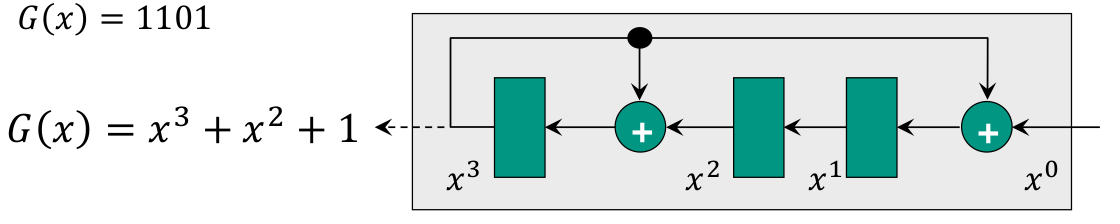
\includegraphics[width=0.33\textwidth]{Schieberegister}\end{figure}

\paragraph{Multiplexing --- Medienzugriff}
\begin{items}
  \item \textbf{Problem}: Link von mehreren Knoten parallel benutzt
   \item \textbf{Varianten}: \\*
  - feste Mediumszuteilung (nach einer Dimension, Punkt-zu-Punkt-Verbindungen) \\*
  - konkurrierende Nutzung \( \to \) Zugriffsorganisation notwendig
  \item \textbf{Dimensionen}: Raum \( r \), Zeit \( t \), Frequenz \( f \), Code \( c \)
  \item \textbf{Wichtig}: Schutzabstände erforderlich
\end{items}

\paragraph{Multiplexing --- Raum}
\begin{items}
  \item Raumeinteilung in Sektoren (zB gerichtete Antennen)
  \item \textbf{Kupfermultiplex}: Zuordnung dedizierter Leitungen
  \item \textbf{Einsatz}: Mobilfunkzellen
  \item Space Division Multiple Access (SDMA)
\end{items}

\paragraph{Multiplexing --- Frequenz}
\begin{items}
  \item \textbf{Prinzip}: verfügbare Bandbreite wird in Frequenzabschnitte unterteilt
  \item \textbf{Vorteile}: \\*
    - keine dynamische Koordination nötig \\*
    - auch für analoge Signale möglich
  \item \textbf{Nachteile}: \\*
    - Bandbreitenverschwendung bei ungleichmäßiger Auslastung \\*
    - unflexibel
  \item \textbf{Einsatz}: DSL
\end{items}

\paragraph{Multiplexing --- Zeit}
\begin{items}
  \item \textbf{Prinzip}: Kanal belegt ganzen Frequenzraum für festgelegte Zeit
  \item \textbf{Vorteile}: \\*
    - nur ein Träger gleichzeitig auf Medium \\*
    - auch bei großer Teilnehmerzahl hoher Durchsatz \\*
  \item \textbf{Nachteil}: genaue Synchronisation nötig
  \item \textbf{Einsatz}: Ethernet, WLAN
  \item \textbf{Hinweis}: Standard-Multiplexverfahren im Folgenden
\end{items}

\paragraph{Multiplexing --- Code}
\begin{items}
  \item \textbf{Prinzip}: alle Stationen zur gleichen Zeit auf gleicher Frequenz \\*
    - \emph{Sender}: verknüpft Signal mit eindeutiger Pseudozufallszahl \\*
    - \emph{Empfänger}: kann mithilfe bekannter Pseudozufallszahlfolge + Korrelations- \\* \phantom{-} \phantom{\( \cdot \)} funktion Originalsignal wiederherstellen
  \item \textbf{Vorteile}: \\*
    - keine Frequenzplanung erforderlich \\*
    - großer Coderaum im Vergleich zu Frequenzraum \\*
    - Vorwärtskorrektur + Verschlüsselung leicht integrierbar
  \item \textbf{Nachteile}: \\*
    - höhere Komplexität wegen Signalregenerierung \\*
    - alle Signale müssen bei Empfänger gleich stark ankommen
  \item \textbf{Einsatz}: UMTS
\end{items}

\paragraph{Zeitmultiplex --- Zufallsstrategien}
\begin{items}
  \item \textbf{Aloha}: zufällige, unabhängige, seltene Sendewünsche \\*
    - gleichzeitiges Senden \( \leadsto \) Kollision
  %\begin{figure}[H]\centering\label{Aloha}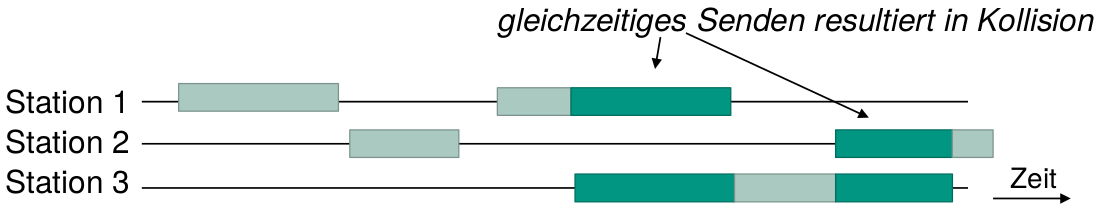
\includegraphics[width=0.33\textwidth]{Aloha}\end{figure}
  \item \textbf{Slotted Aloha}: Verbesserung von Aloha, Erfordert Knotensynchronisation
    \begin{figure}[H]\centering\label{SlottedAloha}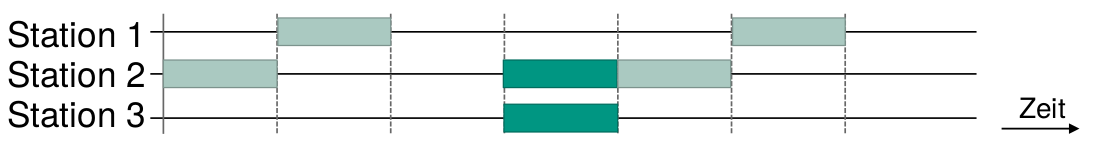
\includegraphics[width=0.33\textwidth]{SlottedAloha}\end{figure}
    \medskip
  \item \textbf{CSMA} (\emph{carrier sense multiple access}): \\*
    - \emph{Prinzip}: Andere nicht unterbrechen während sie reden \\*
    - \emph{listen before talk}: System prüft vor Senden, ob Medium frei ist \\*
    - \emph{Medium belegt}: später erneut versuchen \\*
    - \emph{Medium frei}: Senden \\*
    - \emph{Kollisionen}, wenn mehrere Systeme gleichzeitig zu Senden beginnen
  \item \textbf{CSMA/CD} (\emph{CSMA with collision detection}) \\*
    - \emph{listen while talk}: Kollisionserkennung durch Abhören während des Sendens \\*
    - \emph{Kollision}: Sendungsabbruch, später neu versuchen
\end{items}

\paragraph{Zeitmultiplex --- Umsetzung Ethernet}
\begin{items}
  \item \textbf{Kollision}: \\*
    1. Sendungsabbruch \\*
    2. Sender sendet \emph{Jamming-Signal} \\*
    3. \emph{Backoff-Algorithmus} regelt Sendungswiederholung
  \item \textbf{Vorraussetzungen}: \\*
    - Senden der Rahmen darf nach Signallaufzeit durch Medium und zurück noch nicht \\* \phantom{-} \phantom{\( \cdot \)} fertig sein \\*
    - Mindestlänge für Rahmen (abhängig von Netzausdehnung + Ausbreitungsge- \\* \phantom{-} \phantom{\( \cdot \)} schwindigkeit) erforderlich \\*
    - zu kleiner Rahmen: Auffüllen auf Mindestlänge (\emph{padding})
\end{items}

\newpage

\paragraph{Kollisionsfreier Zugriff --- Prinzip}
\begin{items}
  \item \textbf{Polling}: Kontrolle durch zentralen Knoten \\*
    - Senderecht sequentiell zugewiesen \\*
    - \emph{Nachteil}: koordinierender Knoten nötig, kann ausfallen \\*
    - \emph{Einsatz}: Bluetooth
  \item \textbf{Token Passing}: Senderechtsweitergabe von Knoten zu Knoten \\*
    - \emph{Nachteil}: Knoten können ausfallen \( \to \) Zugriff blockiert \\*
    - \emph{Einsatz}: Token Ring
\end{items}

\paragraph{Kollisionsfreier Zugriff --- Token Ring}
\begin{items}
  \item \textbf{Prinzip}: \\*
    - Systeme physikalisch Punkt-zu-Punkt-verbunden zu Ring \\*
    - Jedes System hat \emph{Vorgänger} und \emph{Nachfolger} \\*
    - Senderechtszuteilung durch zirkulierendes Token\\*
    - Sendendes System nimmt Daten auch wieder vom Ring
    \item Monitor: Endsystem zur Überwachung des Rings, Tokenmanagement (komplex!)
    \item Strukturierte Verkabelung von Gebäuden, Viele Endsysteme möglich
\end{items}
\begin{figure}[H]\centering\label{TokenRing}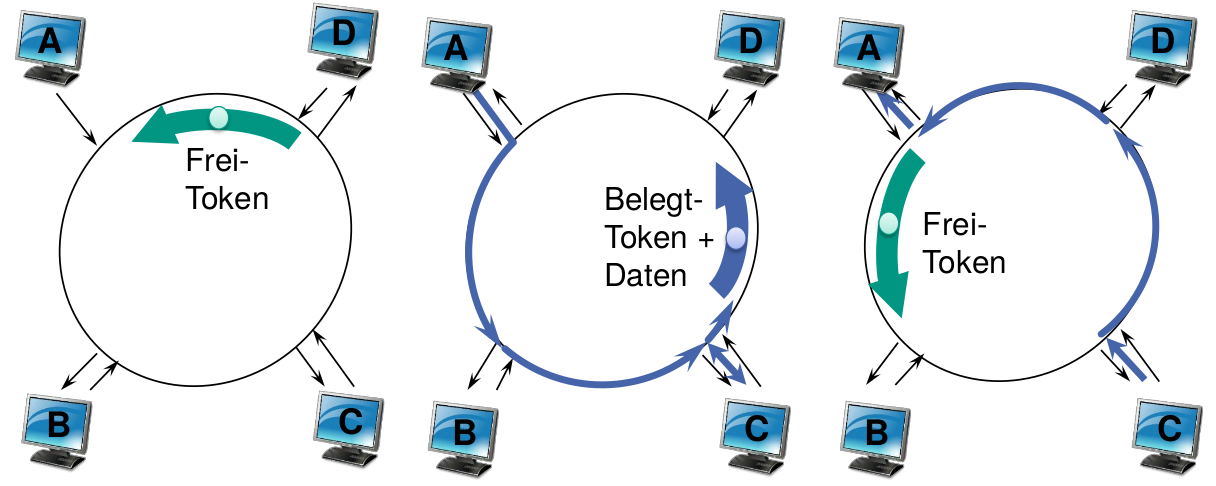
\includegraphics[width=0.33\textwidth]{TokenRing}\end{figure}

\paragraph{Kollisionsfreier Zugriff --- Token Bus}
\begin{items}
  \item \textbf{Prinzip}: \\*
    - Verbindet Vorteile von Ethernet und Token Ring \\*
    - Busverkabelung wie bei Ethernet (robust: Ausfall eines Endsystem für Netz egal) \\*
    - \emph{Garantierte Antwortzeiten} durch zirkulierendes Token
  \item \textbf{Aufbau}: \\*
    - Alle Stationen physikalisch durch Bus verbunden \\*
    - Bildung eines \emph{logischen Rings}
\end{items}
\begin{figure}[H]\centering\label{TokenBus}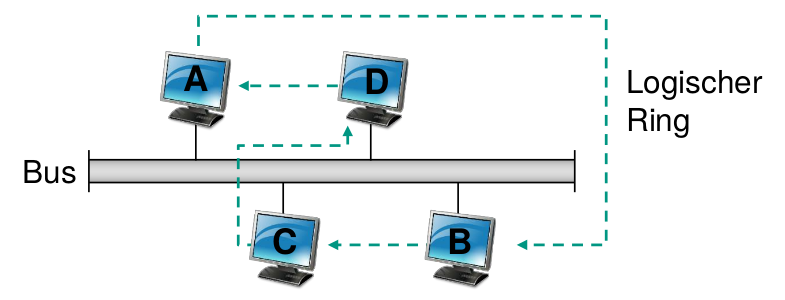
\includegraphics[width=0.33\textwidth]{TokenBus}\end{figure}

\paragraph{Lokale Netze --- MAC-Adressen}
\begin{items}
  \item Theoretisch weltweit eindeutig
  \item Jeder Netzadapter muss in einem lokalen Netz eindeutige MAC-Adresse haben
  \item \textbf{Funktion}: lokal genutzt, um Rahmen von Interface zu benachbartem, physikalisch verbundenem Interface zu übertragen
  \item \textbf{Format}: \\*
    - 48 Bit (24 Bit von IEEE an Hersteller zugewiesen, 24 Bit durchnummeriert) \\*
    - stehen im NIC-ROM, können aber auch per Software gesetzt werden \\*
    - Darstellung meist hexadezimal (zB \code{24-2F-EA-76-CC-28}) \\*
    - Broadcast: \code{FF-FF-FF-FF-FF-FF}
\end{items}

\paragraph{Lokale Netze --- address resolution protocol (ARP)}
\begin{items}
  \item \textbf{Problem}: Welche MAC-Adresse hat nächstes System im eigenen Subnetz?
  \item \textbf{Aufgabe}: MAC-Adresse zu bekannter IP-Adresse ermitteln
  \item \textbf{Prinzip}: dynamisch Adresszuordnungen lernen
  \item \textbf{ARP-Cache}: kleine Tabelle auf jedem System, Einträge bei Bedarf gelernt \\*
    - Eintrag IP + MAC + maximale Lebenszeit (typisch 20 Minuten) 
\end{items}

\paragraph{ARP --- Adressauflösung}
\begin{items}
  \item \textbf{Szenario 1}: \( A \) sendet Datagramm an \( B \) in selbem Subnetz \\*
    - \emph{Fall 1}: ARP-Cache von \( A \) hat Eintrag für \( B \) \\*
      \phantom{-} \( \cdot \) Paket verschicken, Timeout neu setzen \\*
    - \emph{Fall 2}: ARP-Cache von \( A \) hat Eintrag für \( B \) \emph{nicht}: \\*
      \phantom{-} \( \cdot \) Broadcast \emph{ARP-Request} mit IP von \( B \) \\*
      \phantom{-} \( \cdot \) Jeder Knoten liest ARP-Request --- falls eigene IP ARP-Reply \\*
      \phantom{-} \( \cdot \) \( A \) trägt Infos in ARP-Cache ein
  \item \textbf{Szenario 2}: \( A \) sendet Datagramm an \( B \) in anderem Subnetz \\*
    1. \( A \) sendet ARP-Request für Router \( R \) \\*
    2. \( A \) sendet Datagramm an IP von \( B \) und MAC von \( R \) \\*
    3. Router empfängt Datagramm, setzt Ziel-MAC auf \( B \) und Sender-MAC auf \( R \) \\*
    4. Router leitet Datagramm weiter
\end{items}

\paragraph{Lokale Netze --- Ethernet (IEEE 802.3)}
\begin{items}
  \item \textbf{Medienzuteilung}: \\*
    - zeitmultiplex, variabel, zufälliger Zugriff, CSMA/CD\\*
    - Kanal wird logisch in Zeitschlitze fester Länge aufgeteilt \\*
    - Dauer = minimale Rahmenlänge \( \to \) Kollisionserkennung vor Zeitschlitz-Ende\\*
    - Exponentieller Backoff: Warte nach i. Kollision zufällig [0, \( 2^i-1 \)] Zeitschlitze
  \item \textbf{Netztopologie}: Ursprünglich Bus-, heute Sterntopologie (Switches statt Repeatern)
  \item \textbf{Varianten}: [Datenrate][Baseband/Broadband][Medium] (z.B. 10Base5)
   \item Ethernet-Rahmen (immer gleich)\\*
   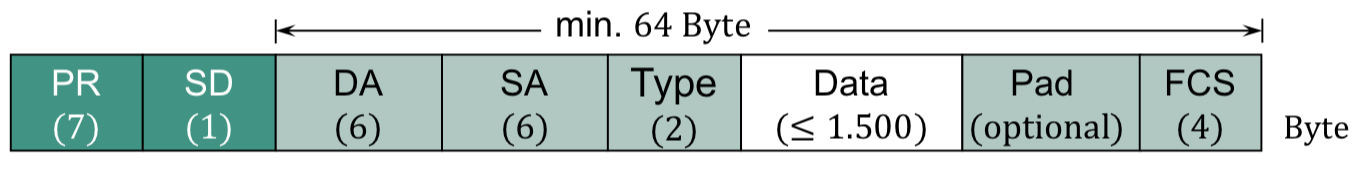
\includegraphics[width=0.4\textwidth]{Ethernet}\\*
   Präambel, Start of Frame Delimiter, Destination Address, Source Address, Type/Length, Data, Padding, Frame Check Sequence
%    - \emph{10Base5}: 10Mbit/s, Baseband, Bustopologie, 10mm Koax \\*
%    - \emph{10Base2}: 10Mbit/s, Baseband, Bustopologie, 5mm Koax
\end{items}
%\begin{figure}[H]\centering\label{EthernetVarianten}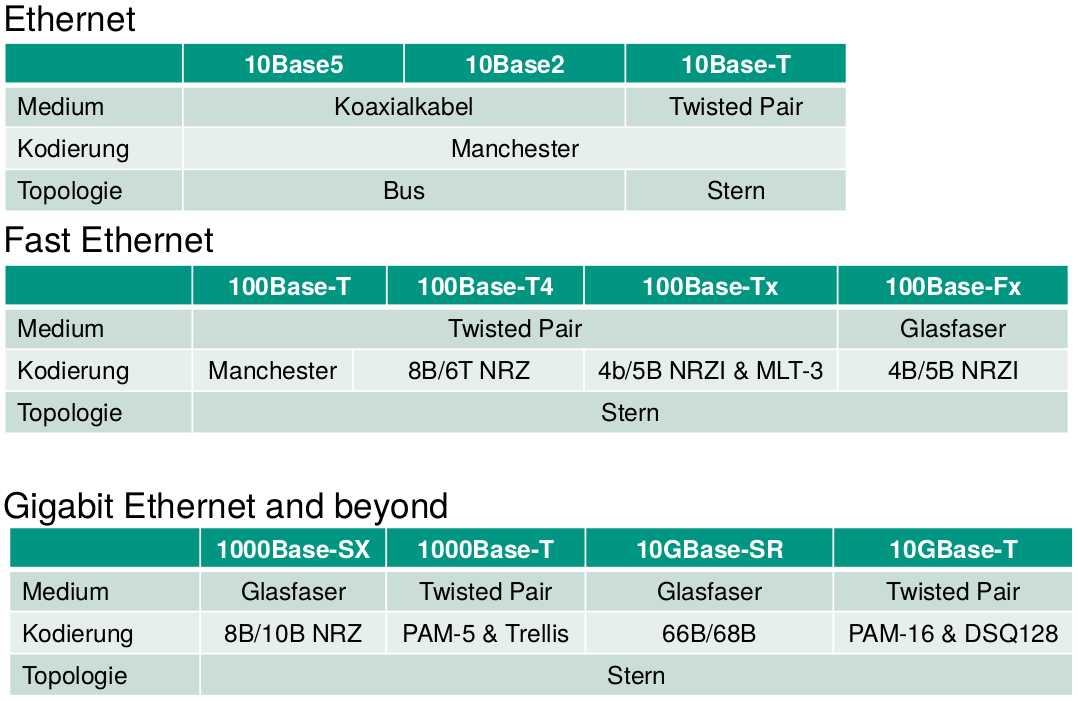
\includegraphics[width=0.33\textwidth]{EthernetVarianten}\end{figure} %i+

\paragraph{Ethernet --- Switches}
\begin{items}
  \item \textbf{Prinzip}: Schicht-2-Netzkopplung (innerhalb \emph{eines} IP-Subnetzes) \\*
    - Leitet Rahmen zwischen Interfaces weiter und puffert sie zwischen\\*
    - Trennung von Inter- und Intranetz-Verkehr \( \to \) Erhöhung Netzkapazität \\*
    - Switches nicht sichtbar für Endsysteme
  \item \textbf{Ziel}: Selbstorganisierte Netzkonfiguration mit Switches
  \item \textbf{Aufgaben}: \\*
    - Schleifenfreie Netztopologie (\emph{spanning tree} Algorithmus) \\*
    - Wege zwischen Endsystemen (selbstlernend; Ziel unbekannt: Fluten)
\end{items}

\paragraph{Ethernet --- Kollisionsdomänen}
\begin{items}
  \item Netzbereich, der von Kollision betroffen ist (gemeinsames Broadcastmedium)
\end{items}
\begin{figure}[H]\centering\label{Kollisionsdomaenen}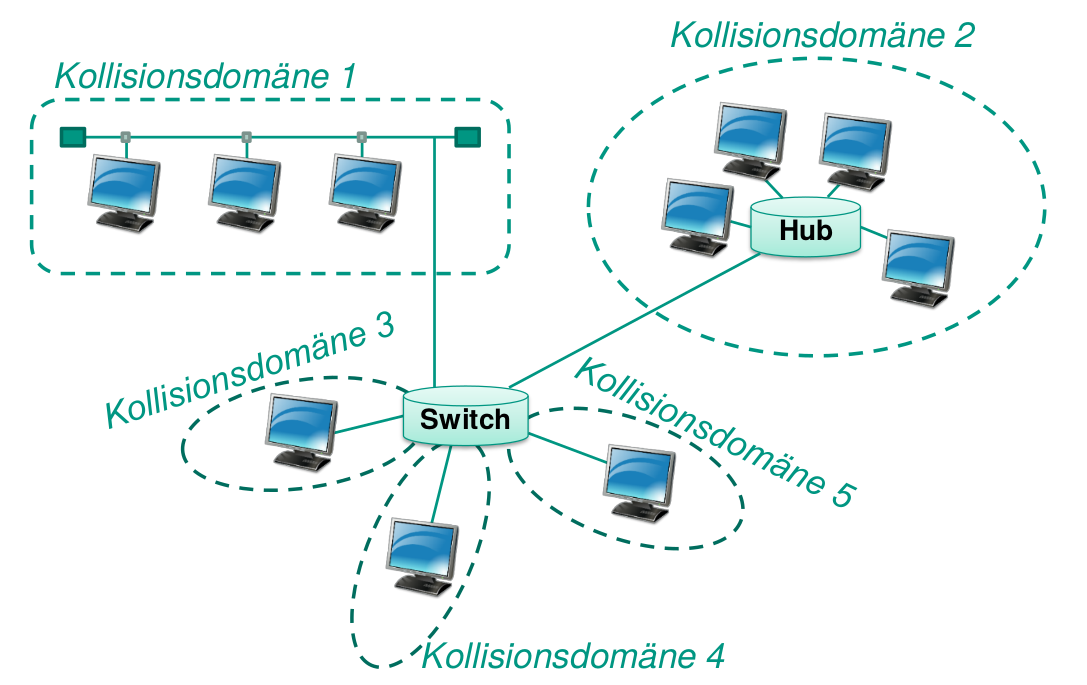
\includegraphics[width=0.33\textwidth]{Kollisionsdomaenen}\end{figure}

\paragraph{virtual local area network (VLAN)}
\begin{items}
  \item \textbf{Idee}: Logische Trennung von Datenverkehr auf Ethernet-Ebene \( \leadsto \) virtuelle Leitung
  \item \textbf{Sicherheit}: \\*
    - Trennung in logische Medien ermöglicht gezielte Systemgruppierung \\*
    - Bessere Kontrolle über Netzstruktur
  \item \textbf{Flexibilität}: \\*
    - Einfache Reorganisation der logischen Medien möglich \\*
    - keine Änderungen an physikalischem Medium (Neuverkabelung) nötig
  \item \textbf{Performance}: Broadcast-Last eines Netzes sinkt, wenn physikalisches Medium in mehrere logische aufgeteilt wird
\end{items}

\paragraph{VLAN --- Interface-basiert}
\begin{items}
	\item Ein einziger physikalischer Switch arbeitet als mehrere virtuelle Switches
	\item Jeweils mehrere Interfaces werden zu einem virtuellen Switch gruppiert
	\smallskip
  \item \textbf{Verkehrsisolation}: Rahmen von einem Interface können nur Interfaces in der gleichen Gruppe erreichen \( \leadsto \) Sicherheit, Performance
  \item \textbf{Flexible Zuweisung}: Interfaces dynamisch anderen VLANs zuordnen
  \item \textbf{Weiterleitung} zwischen VLANs über Routing (oft über in Switch integrierten Router)
  \smallskip
  \item \textbf{Trunks}: Transport von Rahmen zwischen multi-switch-VLANs \\*
    - \emph{VLAN-ID}: Jedes VLAN erhält Kennzeichner \\*
    - Ethernet-Frames werden mit VLAN-ID getaggt \\*
    - Switches entfernen Tagging vor Auslieferung an Endsystem
\end{items}
%\begin{figure}[H]\centering\label{VLAN}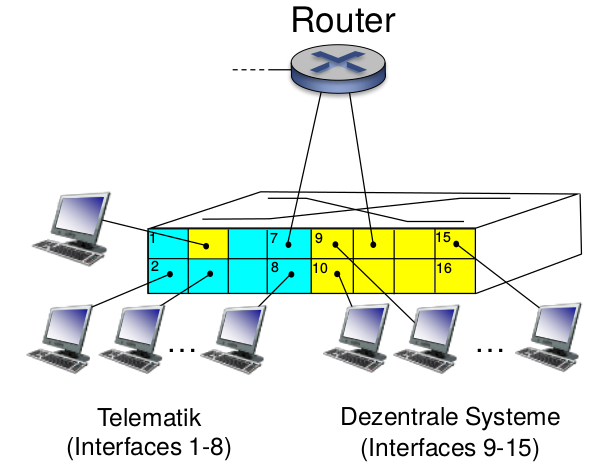
\includegraphics[width=0.33\textwidth]{VLAN}\end{figure}